\documentclass[pdf]{beamer}
\usepackage[utf8]{inputenc}
\usepackage{graphicx}
\usepackage[T1]{fontenc}
\usepackage[francais]{babel}
\usepackage{graphicx}
\usepackage{circuitikz}
\usepackage[squaren, Gray]{SIunits}
\usepackage{sistyle}
\usepackage[autolanguage]{numprint}
\usepackage{pgfplots}
\usepackage{amsmath,amssymb,array}

\usetheme{warsaw}
\mode<presentation>{}

\title{Projet 2 : concevoir un haut-parleur}
\author{Groupe 115.3}
\date{18 juin 2014}

\begin{document}

% =======================================================================
\begin{frame}
\titlepage
\end{frame}


% =======================================================================

\begin{frame}
\frametitle{Introduction et plan de l'exposé}
\begin{figure}[ht!]
    \centering
    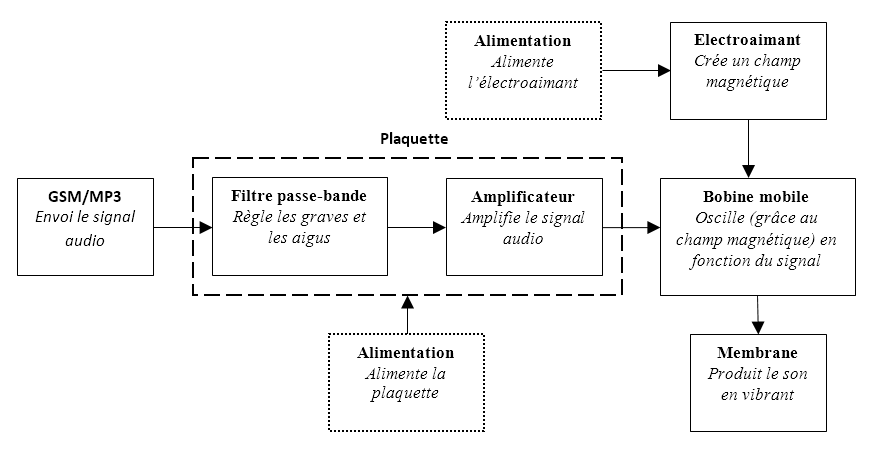
\includegraphics[scale=0.53]{schema_fonctionnel.png}
    \caption{Schéma fonctionnel du haut-parleur}
    \label{schema_fonctionnel}
\end{figure}
\end{frame}

% =======================================================================

\begin{frame}
\frametitle{Dimensionnement du haut-parleur}
\center{Pour le boîtier} \\
\begin{itemize}
\item volume de 25 x 25 x 25 cm
\item matériau MDF 18mm
\item pieds en caoutchouc
\item porte coulissante
\end{itemize}
\center{Pour la membrane} \\
\begin{itemize}
\item diamètre de 17cm
\item matériaux papier et tissus
\end{itemize}
\end{frame}

% =======================================================================

\begin{frame}
\frametitle{Modélisation mécanique du haut-parleur}
\begin{figure}[ht]
\minipage{0.4\textwidth}
\underline{Équation du mouvement}
$$m\fvdd{x}(t) = -k\fv{x}(t) + BLi(t)$$
Hypothèses: 
\begin{itemize}
\item négliger le poids de la bobine
\item négliger le frottement
\end{itemize}
\endminipage\hfill
\minipage{0.4\textwidth}
\underline{Observations importantes}
$$f= \frac{1}{2\pi} \cdot{\sqrt{\frac{k}{m}}}$$
Fréquence de résonance, amplitude du mouvement infini.
\endminipage\hfill
\end{figure}
\end{frame}

% =======================================================================
